%\documentclass[10pt, twocolumn]{article}
%\documentclass[11pt]{article}
%\documentclass[twocolumn,showpacs,preprintnumbers,amsmath,amssymb,prl, superscriptaddress]{revtex4}
%\documentclass[twocolumn, preprintnumbers,amsmath,amssymb,prd, superscriptaddress]{revtex4}
\documentclass[preprintnumbers,amsmath,amssymb,prd,superscriptaddress]{revtex4}
%\documentclass[10pt, preprint,showpacs,preprintnumbers,amsmath,amssymb, superscriptaddress]{revtex4}
%\documentclass[11pt, prd,preprintnumbers,amsmath,amssymb, superscriptaddress]{revtex4}
%\documentclass[11pt, prd,preprintnumbers, amsmath,amssymb, superscriptaddress, nofootinbib, hyperref]{revtex4}

\usepackage{latexsym}
\usepackage{amssymb}
\usepackage{epsfig,amsmath,graphics}
\usepackage{epstopdf}
\usepackage{verbatim}
\usepackage{wasysym}
\usepackage{hyperref}
\usepackage{feynmp-auto} % feynman diagrams
%\usepackage{subfig}
\usepackage[utf8]{inputenc}
\usepackage{xpatch}
\usepackage{xcolor}
\usepackage{mathtools}
\hypersetup{
    colorlinks,
    linkcolor={red!80!black},
    citecolor={green!60!black},
    urlcolor={blue!60!black}
}
\usepackage{appendix}

\newcommand{\Ez}{\mathcal{E}_0}
\newcommand{\Eboom}{\mathcal{E}_\text{boom}}
\newcommand{\OO}{\mathcal{O}}
\newcommand{\LL}{\mathcal{L}}
\newcommand{\HH}{\mathcal{H}}
\newcommand{\TeV}{\text{TeV}}
\newcommand{\GeV}{\text{GeV}}
\newcommand{\MeV}{\text{MeV}}
\newcommand{\keV}{\text{keV}}
\newcommand{\rad}{\text{rad}}
\newcommand{\cm}{\text{cm}}
\newcommand{\angstrom}{\buildrel _{\circ} \over {\mathrm{A}}}
\newcommand{\pslash}{p\hspace{-0.070in}/\,}
\newcommand{\Mpl}{M_{\text{pl}}}
\newcommand{\ket}[1]{\ensuremath{\left|#1\right>}}
\newcommand{\bra}[1]{\ensuremath{\left<#1\right|}}
\newcommand{\braket}[2]{\ensuremath{\left<#1|#2\right>}}
%Large Parentheses
\def\r{\right)}
\def\l{\left(}

\begin{document}

%\preprint{APS/123-QED}

\subsection{Transits}

\paragraph{Ignition Condition.}
Runaway fusion only occurs in the degenerate WD interior where thermal expansion is suppressed as a cooling mechanism.
The outer layers of the WD, however, are composed of a non-degenerate gas and it is therefore essential that a DM candidate penetrate this layer in order to ignite a SN.
We parameterize this by a DM stopping power $(dE/dx)_\text{SP}$, the kinetic energy lost by the DM per distance traveled in the non-degenerate layer, and demand that
\begin{align}
\label{eq:CrustCondition}
  \left( \frac{d E}{d x} \right)_\text{SP} \ll
  \frac{m_\chi v^2_\text{esc}}{R_\text{envelope}},
\end{align}
where $R_\text{envelope} \approx 50 ~\text{km}$ is the width of a WD envelope \cite{KippenhahnWeigert}.

The energy deposited during a continuous heating event such as a DM transit is best described in terms of a linear energy transfer $(dE/dx)_\text{LET}$, the kinetic energy of SM particles produced per distance traveled by the DM.
If these products have a heating length $L_0$ then the relevant energy deposit must at minimum be taken as the energy transferred over the transit distance $L_0$.
Of course, we can always choose to consider energy deposits over a longer segment of the DM trajectory.
Importantly, as per the general condition \eqref{eq:energy_boom_condition} such a deposition is \emph{less} explosive unless $L_0$ is smaller than the trigger size $\lambda_T$.
Thus, we consider the energy deposited in a transit over the larger of these two length scales.
Assuming the energy of the DM is roughly constant over this heating event, the ignition condition for transit heating is:
\begin{align}
\label{eq:transitexplosion}
  \left( \frac{d E}{d x} \right)_\text{LET} \gtrsim
  \frac{\Eboom}{\lambda_T} \cdot \text{max}
  \left\{\frac{L_0}{\lambda_T}, 1 \right\}^2.
\end{align}
Note that the DM stopping power in the non-degenerate layer $(dE/dx)_\text{SP}$ and the linear energy transfer in the degenerate interior $(dE/dx)_\text{LET}$ are possibly controlled by different physics and may have very different numerical values.
In addition, a transit heating event satisfying condition \eqref{eq:CrustCondition} will have negligible energy loss over the parametrically smaller trigger size or heating length $L_0$, validating \eqref{eq:transitexplosion}.

The above argument sums the individual energy deposits along the DM trajectory as though they are all deposited simultaneously.
This is possible if the DM moves sufficiently quickly so that this energy does not diffuse out of the region of interest before the DM has traversed the region.
We therefore require that the diffusion time $\tau_\text{diff} \approx 10^{-12} ~\text{s}$ across a heated region at temperature $T_f$ be larger than the DM crossing-time:
\begin{align}
  \tau_\text{diff} \sim \frac{L^2}{\alpha(T_f)} \gg
  \frac{L}{v_\text{esc}},
\label{eq:SlowDiffusion}
\end{align}
where $\alpha(T)$ is the temperature-dependent diffusivity, and the DM transits at the stellar escape velocity $v_\text{esc} \sim 10^{-2}$.
This condition is more stringent for smaller regions, so we focus on the smallest region of interest, $L = \lambda_T$.
\eqref{eq:SlowDiffusion} is then equivalent to demanding that the escape speed is greater than the conductive speed of the fusion wave front, $v_\text{cond} \sim \alpha(T_f) / \lambda_T$.
Numerical calculations of $v_\text{cond}$ are tabulated in \cite{Woosley}, and indeed condition \eqref{eq:SlowDiffusion} is satisfied for all WD densities.

\paragraph{Event Rate: Wind Scenario.}
The rate of transit events is given by the flux of DM passing through a WD
\begin{align}
  \Gamma_\text{trans} \sim
  \frac{\rho_{\chi}}{m_\chi} R_\text{WD}^2
  \l\frac{v_\text{esc}}{v_\text{halo}}\r^2 v_\text{halo},
\label{eq:TransitFluxCondition}
\end{align}
where $m_\chi$ is the DM mass, $\rho_\chi$ is the DM density in the region of the WD, and $R_\text{WD}$ is the WD radius.
Here $v_\text{halo} \sim 10^{-3}$ is the virial velocity of our galactic halo, and the transit rate contains an $(v_\text{esc}/v_\text{halo})^2 \sim 100$ enhancement due to gravitational focusing.

\subsection{Collisions and Decays}

\paragraph{Ignition Condition.}
For a point-like DM-DM collision or DM decay event releasing particles of heating length $L_0$, ignition will occur if the total energy in SM products satisfies condition~\eqref{eq:energy_boom_condition}.
Such an event will likely result in both SM and dark sector products, so we parameterize the resulting energy in SM particles as a fraction $f_\text{SM}$ of the DM mass.
For non-relativistic DM, the DM mass is the dominant source of energy and therefore $f_\text{SM} \lesssim 1$ regardless of the interaction details.
With this parameterization, a single DM-DM collision or DM decay has an ignition condition:
\begin{equation}
\label{eq:coldecay}
  m_\chi f_\text{SM}  \gtrsim \Eboom \cdot \text{max} \left \{\frac{L_0}{\lambda_T}, 1 \right \}^3.
\end{equation}
We are thus sensitive to DM masses $m_\chi \gtrsim 10^{16} ~\GeV$.

However, there is the possibility if DM is captured in the WD that allows collisions or decays of lower mass DM to ignite the star. 
Multiple DM-DM collisions or decays in a sufficiently small region can occur rapidly enough to be counted as a single heating event.
This is similar in nature to a transit heating event, where multiple scatters across a transit length $\lambda_T$ can release an energy $\Eboom$ and satisfy \eqref{eq:transitexplosion} even if any individual scatter is not explosive by itself.   
If a single DM-DM collision is unable to ignite the star, the sum total of the energy released in many collisions can still result in a SN if
\begin{equation}
\label{eq:multcolboom}
 m_\chi f_\text{SM} \gtrsim \frac{\Eboom}{N_\text{mult}} \cdot \text{max} \left \{\frac{L_0}{\lambda_T}, 1 \right \}^3, ~~~~ N_\text{mult} \gtrsim 1,
\end{equation}
We define $N_\text{mult}$ as the number of collisions within a region of size $\text{max}\{\lambda_T,L_0\}^3$ (or smaller) during a diffusion time $\tau_\text{diff}$.
This necessarily depends on additional DM parameters and the evolution of the captured DM in the star. 
These are discussed in detail below. 

\paragraph{Event Rate: DM Wind.}
For the remainder of this section, all numerical quantities are evaluated assuming a WD lifetime $\tau_\text{WD} \sim 5 ~\text{Gyr}$ and central WD density $n_\text{ion} \sim 10^{31} ~\cm^{-3}$. 
At this density, the relevant WD parameters are approximately: 
\begin{equation}
M_\text{WD} \approx 1.25 ~M_{\astrosun}, ~~~~ R_\text{WD} \approx 4000 ~\text{km}, ~~~~ v_\text{esc} \approx 2 \times 10^{-2}. 
\end{equation}
We also assume a typical WD temperature $T \sim \text{keV}$.
DM that is not captured traverses the WD in $R_\text{WD}/v_\text{esc} \approx 0.1 ~\text{s}$, and the rate of DM-DM collisions within the WD parameterized by cross-section $\sigma_{\chi \chi}$ is:
\begin{align}
  \Gamma_\text{ann}
  \sim \l \frac{\rho_\chi}{m_\chi} \r^2 \sigma_{\chi \chi} \l \frac{v_\text{esc}}{v_\text{halo}}\r^3 v_\text{halo} R_\text{WD}^3. 
  \label{eq:collisionDM}
\end{align}
Similarly the net DM decay rate inside the WD parameterized by a lifetime $\tau_\chi$ is:
\begin{align}
 \Gamma_\text{decay}
   \sim \frac{1}{\tau_\chi} \frac{\rho_{\chi}}{m_\chi} \l \frac{v_\text{esc}}{v_\text{halo}}\r R_\text{WD}^3.
  \label{eq:decayDM}
\end{align}

\paragraph{Event Rate: DM Capture.}
For the DM to be captured in a WD, it must lose energy $\sim m_\chi v^2$, where $v$ is the relative DM velocity (in the rest frame of the WD) asymptotically far away.
Properly, this DM velocity is described by a (boosted) Maxwell distribution peaked at the galactic virial velocity $v_\text{halo} \sim 10^{-3}$. 
Since typically $v \ll v_\text{esc}$, the DM has initial velocity $v_\text{esc}$ in the star and must lose a fraction $(v/v_\text{esc})^2$ of its energy to become captured. 

The physics of DM capture can be made more precise for a specific interaction.
Consider a spin-independent, elastic scattering off ions with cross section $\sigma_{\chi A}$. 
Assuming $m_\text{ion} \ll m_\chi$, the typical momentum transfer in an elastic scatter is $q \sim \mu_{A} v_\text{esc} \approx 200 ~\MeV$, where $\mu_{A} \sim m_\text{ion}$ is the reduced mass of the DM-nuclei system. 
This corresponds to an energy transfer $q^2/m_\text{ion} \sim m_\text{ion} v_\text{esc}^2 \approx 10 ~\MeV$. 
The average number of DM scatters during a full transit of the WD is simply a ratio of the mean free path to the size of the WD
\begin{equation}
N_\text{scat} \sim n_\text{ion} \sigma_{\chi A} R_\text{WD}.
\end{equation}
If $N_\text{scat} < 1$, then $N_\text{scat}$ is the probability for a \emph{single} scatter to occur during the transit. 
Thus, DM with initial velocites less than
\begin{equation}
\label{eq:capture}
v_\text{cap}^2 \sim v_\text{esc}^2 \l \frac{m_\text{ion}}{m_\chi} \r \text{max}\{N_\text{scat} ,1\}.
\end{equation}
will be captured in the WD. 
A detailed calculation of the rate of DM capture \cite{Gould} yields  
\begin{equation}
\Gamma_\text{cap} \sim \Gamma_\text{trans} \cdot \text{min}\{N_\text{scat}, 1\} \l \frac{v_\text{cap}}{v_\text{halo}} \r^2.
\end{equation}
Here we assume $v_\text{cap} < v_\text{halo}$; otherwise, the capture rate is simply $\Gamma_\text{trans}$. 
%Evidently, the assumption that the scatters responsible for slowing the DM are not sufficient to blow up the WD \eqref{eq:transitexplosion} is a valid one for cross sections
%\begin{equation}
%\sigma_{\chi A} < \l \frac{\Eboom}{\lambda_T} \r \l \frac{1}{m_\text{ion} v_\text{esc}^2} \r \l \frac{1}{n_\text{ion}} \r \approx 10^{-8} ~\cm^2,
%\end{equation}
Since the momentum transfer $q$ is roughly of order the inverse nuclear size, it is reasonable to expect the DM coherently scatters off all nucleons in the nucleus. 
Indeed, the average per-nucleon cross section (spin-independent) is
\begin{equation}
\sigma_{\chi A} = A^2 \l \frac{\mu_{A}}{\mu_{n}}\r^2 F^2(q) \sigma_{\chi n},
\end{equation}
where $F^2(q) \approx 0.1$ is the Helm form factor \cite{LUX thesis}.  
We can compare the cross section sufficient for capture \eqref{eq:capture} to the limits from direct detection experiments.
%In addition, the assumption that the DM mean free path is smaller than the size of the WD is valid for
%\begin{equation}
%\sigma_{\chi n} \gtrsim 10^{-43} ~\cm^2.
%\end{equation}
Currently, the bound on spin-independent DM nuclear elastic scatters from XENON 1T is
\begin{equation}
\label{eq:xenon}
\sigma_{\chi n} < 10^{-45} ~\text{cm}^2 \l \frac{m_\chi}{10^3 ~\GeV} \r.
\end{equation}
It is interesting that any DM candidate whose scattering cross section barely avoids the direct detection constraint can be efficiently captured in a WD, $v_\text{cap} \approx 0.5 ~v_\text{halo}$. 

If the DM is captured, it eventually thermalizes to an average velocity
\begin{equation}
v_\text{th} \sim \sqrt{\frac{T}{m_\chi}} \approx 10^{-12} \l \frac{m_\chi}{10^{16} ~\GeV}\r^{-1/2}
\end{equation}
and settles at the thermal radius
\begin{align}
R_\text{th} \sim \l \frac{T}{G m_\chi \rho_\text{WD}}\r^{1/2} \approx 0.1 ~\cm \l \frac{m_\chi}{10^{16} ~\GeV}\r^{-1/2},
\end{align}
where its kinetic energy balances against the gravitational potential energy of the (enclosed) WD mass. 
For simplicity we take a constant WD density $\rho_\text{WD} \sim n_\text{ion} m_\text{ion}$ within $R_\text{th}$.
Of course, the timescale to reach thermalization depends on the nature of the DM-SM interaction.
This has been explicitly calculated in the case that the DM loses energy via elastic nuclear scatters, see \cite{Tinyakov}. 
First, the DM passes through the WD many times before the size of its orbit becomes fully contained within the star.
This occurs after a time
\begin{equation}
t_1 \sim \l \frac{m_\chi}{m_\text{ion}} \r^{3/2} \frac{R_\text{WD}}{v_\text{esc}} \frac{1}{N_\text{scat}} \frac{1}{\text{max}\{N_\text{scat}, 1\}^{1/2}} \approx 2 \times 10^{3} ~\text{yr} \l \frac{m_\chi}{10^{10} ~\GeV} \r^{3/2} \l \frac{\sigma_{\chi A}}{10^{-38} ~\cm^2} \r^{-3/2}. 
\end{equation}
Note that this stage is relevant only if the energy loss after a single transit is does not exceed $\sim m_\chi v_\text{esc}^2$:
\begin{equation}
\l \frac{m_\text{ion}}{m_\chi} \r \text{max}\{N_\text{scat},1\} < 1. 
\end{equation}
This is the case for any cross sections which satisfy the XENON bound \eqref{eq:xenon}. 
Subsequently, the DM completes many orbits within the star until dissipation from elastic scatters reduces the orbital size to the thermal radius.
This occurs after a characteristic time
\begin{equation}
t_2 \sim \l \frac{m_\chi}{m_\text{ion}} \r \frac{1}{n_\text{ion} \sigma_{\chi A}} \frac{1}{v_\text{ion}} \approx 30 ~\text{yr} \l \frac{m_\chi}{10^{10} ~\GeV} \r \l \frac{\sigma_{\chi A}}{10^{-38} ~\cm^2} \r^{-1}. 
\end{equation}
where $v_\text{ion} \sim \sqrt{\frac{T}{m_\text{ion}}}$ is the thermal velocity of ions. 
%If instead the DM rapidly loses energy in the star, we expect this time to be of order
%\begin{align}
%\label{eq:tdrift}
%  t_\text{settle} \sim \frac{R_\text{WD}}{v_\text{th}}
 % \approx 50 ~\text{yr} \l \frac{m_\chi}{10^{16} ~\GeV} \r^{1/2}. 
%\end{align}
Thus, DM will only settle at the thermal radius if the total thermalization time is shorter than the age of the WD:
\begin{equation}
t_1 + t_2 < \tau_\text{WD}.
\end{equation}

We now turn towards the rate of DM-DM collisions for captured DM. 
Ultimately, the most interesting constraint in the capture scenario will be from the focusing of annihilations during self-gravitational collapse of a DM cloud at the thermal radius.
However, we first carefully examine the effect of annihilations on the evolution of captured DM. 
To begin, the settling DM constitutes a number density of DM throughout the WD volume as well as outside the star. 
%\begin{equation}
%n(r) \sim \frac{\Gamma_\text{cap}}{r^2 v(r)}.
%\end{equation}
We can compare the total rate of annihilations of infalling DM to the rate of DM capture.  
This annihilation rate is ultimately dominated by the DM density inside the star with orbits near the thermal radius
\begin{equation}
\label{eq:infallrate}
\Gamma_\text{infall} \sim \frac{\Gamma_\text{cap}^2 \sigma_{\chi \chi}}{R_\text{th} v_\text{th}}.
\end{equation}
Thus, depletion of the infalling DM can be ignored as long as
\begin{equation}
\label{eq:steadycollect}
\Gamma_\text{infall} < \Gamma_\text{cap}.
\end{equation}
Note for the rest of this section, we will evaluate all numerical quantities assuming efficient capture of the DM: $\Gamma_\text{cap} \sim \Gamma_\text{trans}$. 
%As such, condition \eqref{eq:steadycollect} is independent of $m_\chi$ and yields an upper bound on the cross section $\sigma_{\chi \chi} < 10^{-13} ~\text{cm}^2$. 
After a settling time has passed, DM will begin steadily accumulating at $R_\text{th}$.
If \eqref{eq:steadycollect} is satisfied, the accumulation rate is roughly the same as the capture rate. 
However, this density of accumulating DM is also depleting due to annihilations. 
Eventually, these two rates become comparable and there is an equilibrium number of DM particles
\begin{align}
N_\text{eq} \sim \l \frac{\Gamma_\text{cap} R_\text{th}^3}{\sigma_{\chi \chi} v_\text{th}} \r^{1/2} \approx 10^{19} \l \frac{m_\chi}{10^{16} ~\GeV} \r^{-1} \l \frac{\sigma_{\chi \chi}}{10^{-30} ~\cm^2} \r^{-1/2} \l \frac{\rho_\chi}{0.4 ~\GeV/\cm^3} \r^{1/2}.
\end{align}
Of course, there is no guarantee that this equilibrium is achieved within the age of the WD. 
In that case, annihilations can be ignored and the total number of DM particles accumulated is simply
\begin{align}
N_\text{life} &\sim \Gamma_\text{cap} \tau_\text{WD} \approx 10^{29}  \l \frac{m_\chi}{10^{16} ~\GeV} \r^{-1} \l \frac{\rho_\chi}{0.4 ~\GeV/\cm^3} \r
\end{align}
As expected, the total \emph{mass} of DM that the WD can possibly accumulate $N_\text{life} m_\chi \approx 10^{45} ~\GeV$ is independent of $m_\chi$. 
However, if the collected mass of DM at the thermal radius ever exceeds the WD mass within this volume, then there is the possibility of self-gravitational collapse of the DM.
The critical number of DM particles needed for collapse is given by
\begin{align}
\label{eq:Ncore}
    N_\text{crit} \sim \frac{\rho_\text{WD} R^3_\text{th}}{m_\chi} \approx 10^{12} \l \frac{m_\chi}{10^{16} ~\GeV} \r^{-5/2}.
\end{align}
This can only be achieved if the time to collect a critical mass of DM is shorter than the time for annihilations to deplete this mass sufficiently \emph{and} shorter than the WD lifetime. 
Thus the condition for collapse is:
\begin{equation}
\label{eq:collapsecondition}
N_\text{crit} < N_\text{eq}, ~~~~ N_\text{crit} < N_\text{life}. 
\end{equation}
Evidently, DM masses less than $\sim 10^{6} ~\GeV$ do not have enough time within the age of the WD to collect a number $N_\text{crit}$ and begin a collapse.
At a given radius $r$, the time it takes for the DM to free-fall an $\OO(1)$ fraction of this distance is roughly
\begin{equation}
\label{eq:freefalltime}
t_\text{ff} \sim \frac{r}{v_\text{ff}}, ~~~~ v_\text{ff} \sim \sqrt{\frac{G N m_\chi}{r}},
\end{equation}
while the timescale for self-gravitational collapse at the thermal radius is independent of DM mass:
\begin{align}
\label{eq:collapsetime}
  t_\text{col} \sim \frac{R_\text{th}}{v_\text{th}} \sim \sqrt{\frac{1}{G \rho_\text{WD}}} \approx 0.1 ~\text{s}.
\end{align}
Of course, it is possible that the DM initially remains thermalized while collapsing due to sufficiently strong DM-SM interactions. 
In the case of elastic nuclear scatters the DM loses a fraction $\sim m_\text{ion}/m_\chi$ of its energy per collision, so the DM is free-falling at the thermal radius as long as
\begin{equation}
\sigma_{\chi A} \lesssim \frac{1}{n_\text{ion} R_\text{th}} \l \frac{m_\chi}{m_\text{ion}}\r \approx 10^{-30} ~\cm^2 \l \frac{m_\chi}{10^6 ~\GeV} \r^{3/2}.
\end{equation}
It is straightforward to see that this is the case for any cross sections which satisfy the XENON bound \eqref{eq:xenon}.
Annihilations in the collapsing DM density become significant when the free-fall time is of order the time for a single DM to annihilate.
This occurs at the characteristic radius
\begin{align}
R_{\chi \chi} \sim \sqrt{N_\text{crit} \sigma_{\chi \chi}} \approx 10^{-9} ~\cm  \l \frac{m_\chi}{10^{16} ~\GeV} \r^{-5/4} \l \frac{\sigma_{\chi \chi}}{10^{-30} ~\cm^2} \r^{1/2}. 
\end{align}
As a check of consistency, such a collapse of the accumulated DM in the WD is only sensible if
\begin{align}
\label{eq:xicondition}
R_{\chi \chi} < R_\text{th},
\end{align}
which is trivially satisfied if both \eqref{eq:steadycollect} and \eqref{eq:collapsecondition} are true. 
The number (and mass) of collapsing DM is depleting by an $\OO(1)$ fraction at a distance $R_{\chi \chi}$, while below this radius the number is determined by:
\begin{equation}
\frac{dN(r)}{dr} \sim \frac{N(r)^2}{r^3} \sigma_{\chi \chi}.
\end{equation}
Of course the enclosed WD mass is also dropping by $M_\text{WD}(r) \propto r^3$ during the collapse, so if $N(r)$ depletes as a stronger function of radius then the collapse will halt below $R_{\chi \chi}$. 

We also briefly mention the possibility that the number of DM particles initially collapsing can be greater than $N_\text{crit}$. 
This is the case if captured DM passes through the thermal radius even before sufficiently slowing down to thermal velocity, as is the case for DM thermalizing via elastic scatters. 
Once the accumulated DM reaches $N_\text{crit}$, evolution of the DM profile can either be collapse or further collection.
The later occurs if the time for collapse is greater than time to collect a critical number of DM particles:
\begin{equation}
N_\text{crit} < \Gamma_\text{cap} t_\text{col}.
\end{equation}
If $\Gamma_\text{cap} \sim \Gamma_\text{trans}$, this is true for DM masses above $\sim 10^{17} ~\GeV$. 
Here the DM cloud at $R_\text{th}$ will continue to collect more DM until a saturation number $\sim N_\text{crit}^{1/3} (\Gamma_\text{cap} t_\text{col})^{2/3}$ greater than $N_\text{crit}$, at which point the timescale for free-fall matches the timescale for collection.

There are two potential evolutions of the captured DM: either the DM collapses or it does not. 
In the later case, either the DM has reached its equilibrium number at the thermal radius or is still continuing to accumulate, not yet having the critical mass necessary for collapse within its lifetime:
\begin{equation}
\label{eq:nocollapseann}
\text{min}\{N_\text{eq}, N_\text{life}\} < N_\text{crit}.
\end{equation}
First we see if this scenario allows for any meaningful constraints. 
The number of collisions that can be counted as a single heating event is roughly
\begin{equation}
\label{eq:nocollapse}
N_\text{mult} \sim \l \frac{\text{min}\{N_\text{eq}, N_\text{life}\}}{R_\text{th}^3} \r^2 \sigma_{\chi \chi} v_\text{th} L_\text{heat}^3 \tau_\text{diff}, ~~~~ L_\text{heat} \equiv \text{max}\{\lambda_T, L_0\}. 
\end{equation}
Even in the ``best-case" scenario of efficient capture and $L_0 \sim \lambda_T$, we find there is no parameter space $\{m_\chi, \sigma_{\chi \chi}\}$ where both \eqref{eq:nocollapseann} and \eqref{eq:multcolboom}---with $N_\text{mult}$ given by \eqref{eq:nocollapse}---are simultaneously satisfied. 

We instead turn our attention to collapsing DM, characterized by \eqref{eq:collapsecondition}. 
Of course, the number of collisions $N_\text{mult}$ that can be counted as a single heating event depends on where we examine the collapse. 
In general, this is given as an integral of the annihilation rate
\begin{equation}
\label{eq:capintegral}
N_\text{mult} \sim \int \l \frac{N}{r^3}\r^2 \sigma_{\chi \chi} \text{min}\{L_\text{heat}, r\}^3 dr
\end{equation}
integrating over the distance fell within a fixed time interval $\tau_\text{diff}$. 
The expectation is that there exists an optimal value of the lower radius at which $N_\text{mult}$ is maximized.
We denote this as $R_*$. 
However, even without knowing the details of this optimum choice, we can calculate \eqref{eq:capintegral} by considering the following limits. 
If the free-fall time \eqref{eq:freefalltime} at a distance of order $R_*$ is much larger than the diffusion time, the annihilation rate can be approximated as constant over a time $\tau_\text{diff}$.
If this free-fall time is instead much smaller than the diffusion time, the annihilation rate is a rapidly increasing function over the interval $\tau_\text{diff}$.
Therefore, \eqref{eq:capintegral} is approximated by the peak value of the annihilation rate (which is maximized at $R_*$) multiplied by the time spent at this peak (which is the time to free-fall $\sim R_*$).
Considering both these possibilities, the maximum value of \eqref{eq:capintegral} is of the form: 
\begin{equation}
\label{eq:nmulti}
N_\text{mult} \sim \l \frac{N}{R_*^3}\r^2  \sigma_{\chi \chi} v_\text{ff} ~\text{min}\{L_\text{heat}, R_*\}^3 ~\text{min}\left \{\tau_\text{diff}, \frac{R_*}{v_\text{ff}}\right \},
\end{equation}

The questions is: what is $R_*$?
Ultimately, the answer depends on the parameters $m_\chi$ and $\sigma_{\chi \chi}$. 
Suppose $\sigma_{\chi \chi}$ is independent of velocity or position.
In this case, the scaling is such that $N_\text{mult}$ is maximized at the smaller of the two scales $R_* \sim \text{min}\{R_{\chi \chi}, L_\text{heat}\}$. 
However, there may be some stabilizing pressure which prevents the DM from collapsing below a certain radius.
This is reasonable to expect in the case of composite DM, although such a stable radius would depend on unknown physics. 
Famously, gravity itself provides such a ``pressure", arresting collapses below the Schwarzschild radius by the formation of a black hole:
\begin{equation}
R_\text{BH} \sim G N_\text{crit} m_\chi \approx 5 \times 10^{-24} ~\cm \l \frac{m_\chi}{10^{16} ~\GeV} \r^{-3/2}.
\end{equation}
Of course, this choice of radius will necessarily change for a specific model that relates $\sigma_{\chi \chi}$ to velocity in some way. 
For instance if $\sigma_{\chi \chi} \propto 1/v$ then the optimum radius is instead just $R_* \sim R_{\chi \chi}$.
Regardless, it ends up being the case that for most cross sections and DM masses which satisfy the collapse condition \eqref{eq:collapsecondition}, the scale $R_{\chi \chi}$ is less than $10^{-5} ~\cm$. 
Thus for the sake of simplicity, we look at the collapse at a radius
\begin{equation}
R_* = \text{max}\{R_{\chi \chi}, R_\text{BH}\}.
\end{equation}
As expected $N_\text{mult}$ is at most $N_\text{crit}$, the initial number of DM particles collapsing, if $R_* \sim R_{\chi \chi}$.  
If the DM stabilizes into a BH, the condition that not even a \emph{single} collision occurs during the collapse to $R_\text{BH}$ is simply
\begin{equation}
\sigma_{\chi \chi} < G^2 m_\chi^2. 
\end{equation}
This is the most stringent bound that can be placed on DM masses greater than $\Eboom$, for which a single collision is capable of igniting the star. 

Finally, we examine the decay rate of captured DM in the WD. 
Of course, this rate is proportional to the number of DM particles within the WD at any given instance.  
In the wind scenario \eqref{eq:decayDM}, this number is given by $\sim (\Gamma_\text{trans} \times 0.1 ~\text{s})$.  
In the capture scenario, the number of DM particles available for decay is instead determined by the settling time inside the WD. 
Note that for DM masses above $\Eboom$, it is the case that gravitational collapse will occur within the age of the WD, i.e. $N_\text{crit} < N_\text{life}$. 
If the DM is captured via elastic scatters, the rate of decays is given by
\begin{equation}
\Gamma_\text{decay} \sim  \frac{1}{\tau_\chi} \Gamma_\text{cap} t_2
\label{eq:decayDMcap}
\end{equation}
We see that if the scattering cross section is sufficiently large such that $N_\text{scat} >1$, then \eqref{eq:decayDMcap} is independent of $\sigma_{\chi A}$ and scales inversely with $m_\chi$ just as \eqref{eq:decayDM} does. 
Thus in this regime, the rate of captured DM decays in the WD is simply enhanced by a numerical factor $\sim 10^{7}$ compared to the rate of transiting ``wind" decays.  
Lastly, we have checked that the enhancement of the DM number in the star is never sufficient to yield novel bounds on the DM lifetime if multiple decays are required.

\subsection{Constraints: Capture Scenario}

We now turn towards constraints on DM-DM collisions in the capture scenario.
We do not explicitly show the constraints on DM lifetimes since, as stated in Section \ref{sec:previous}, the resulting bounds are simply that of the wind scenario enhanced by a factor $\sim 10^{7}$. 
In Figure \ref{fig:multicapture}, we derive the constraints on $\sigma_{\chi \chi}$ due to the observation of a single $1.25 ~ M_{\astrosun}$ in our local DM density. 
We distinguish between whether a single collision can blow up the WD or multiple collisions are required, although both bounds are derived from the focusing of annihilations during gravitational core collapse of DM in the star.
Here we have additionally assumed that the DM is efficiently captured ($\Gamma_\text{cap} \sim \Gamma_\text{trans}$), and that the settling time is less than the WD lifetime.
We also take the DM collapse to be stabilized by formation of a BH.
The results of Figure \ref{fig:multicapture} are valid for any SM annihilation products which deposit their energy compactly upon release within the trigger size $\lambda_T$ \textcolor{blue}{see discussion in section 3}. 
\begin{figure}
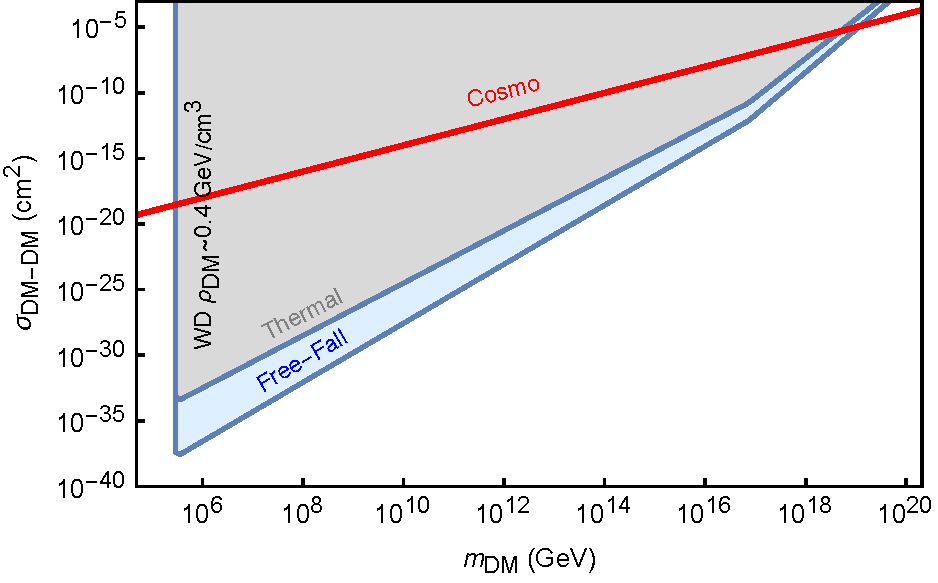
\includegraphics[scale=.35]{multicollision.pdf}
\caption{Constraints on DM-DM annihilation cross-section into SM particles which deposit their energy compactly within a trigger size $\lambda_T$ during self-gravitational collapse in a WD. Bounds come from observation of a single $1.25~M_{\astrosun}$ WD assuming efficient capture of the DM and settling time (see text). We also take the DM collapse to be stabilized by formation of a BH.}
\label{fig:multicapture}
\end{figure}

As per the discussion of Section \ref{sec:previous}, it is straightforward to specify these constraints to DM which is captured by elastic scatters. 
For this, we consider a generic class of heavy WIMP (``WIMPzilla") DM models. 
In particular, suppose the DM scatters off nuclear targets through Z boson exchange, with a per-nucleon cross section
\begin{equation}
\label{eq:Zscattering}
\sigma_{\chi n} \sim \frac{G_F^2 \mu_{\chi n}^2}{2\pi} Y^2 \left [\frac{(A-Z) - (1-4 \sin^2{\theta_W})Z}{A} \right ]^2 \approx 2 \times 10^{-39} ~\cm^2,
\end{equation}
where $G_F$ is the Fermi constant and $Y$ is the hyper-charge of the DM. 
Of course in order to evade direct detection constraints \eqref{eq:xenon}, such a DM must have a mass greater than $m_\chi \gtrsim 10^{10} ~\GeV$. 
It is natural to expect such a DM has an annihilation cross section into electroweak gauge bosons.
DM candidates of this kind can easily arise in theories of physics BSM, e.g. heavy sneutrino DM, ``GUTzilla", etc. 
A naive estimate for the WIMPzilla annihilation cross section is simply
\begin{equation}
\sigma_{\chi \chi} v \sim \frac{1}{8\pi} \frac{g^4}{m_\chi^2} ~~ (\text{naive}).
\end{equation}
However, the cross section will generally larger, e.g. due to a Sommerfeld enhancement. 
There may also be an upper limit on the annihilation cross section, the so-called unitarity limit, if the DM is ``point-like" in nature:
\begin{equation}
\sigma_{\chi \chi} \lesssim \frac{4 \pi}{m_\chi^2} \frac{1}{v} ~~ (\text{unitarity}).
\end{equation}
W and Z bosons decay predominantly to quarks with a decay length of order
\begin{equation}
\delta_W \sim \frac{8\pi}{g^2 m_W} \l \frac{m_\chi}{m_W} \r \sim 10^{-6} ~\cm \l \frac{m_\chi}{10^{10} ~\GeV} \r. 
\end{equation}
Evidently, DM masses $m_\chi > 10^{11}$ will have a decay length larger than the trigger size of a $1.25~M_{\astrosun}$ WD.
However, we expect that at such high energies there should be a considerable branching fraction of the DM-DM annihilations directly into quark-antiquark pairs \textcolor{blue}{check with expert}. 
Thus, since hadrons stop efficiently in the WD medium, the heating length for WIMPzilla annihilations is simply $\lambda_T$. 
\textcolor{blue}{elaborate.}
Note that for such models, the timescale for DM to settle at the thermal radius now becomes an important constraint. 
In particular, we find that a WIMPzilla of mass $\sim 10^{17} ~\GeV$ has a settling time $t_1$ of order $\sim 5 ~\text{Gyr}$. 
This is coincidentally also the mass threshold where a single annihilation can release sufficient energy to ignite a $1.25~M_{\astrosun}$ WD. 
For simplicity we only look at the constraints derived from considering multiple annihilations of WIMPzilla during gravitational collapse---this is done in Figure \ref{fig:Gutzilla}.
Such bounds are complementary to those obtained in the wind scenario.  
\begin{figure}
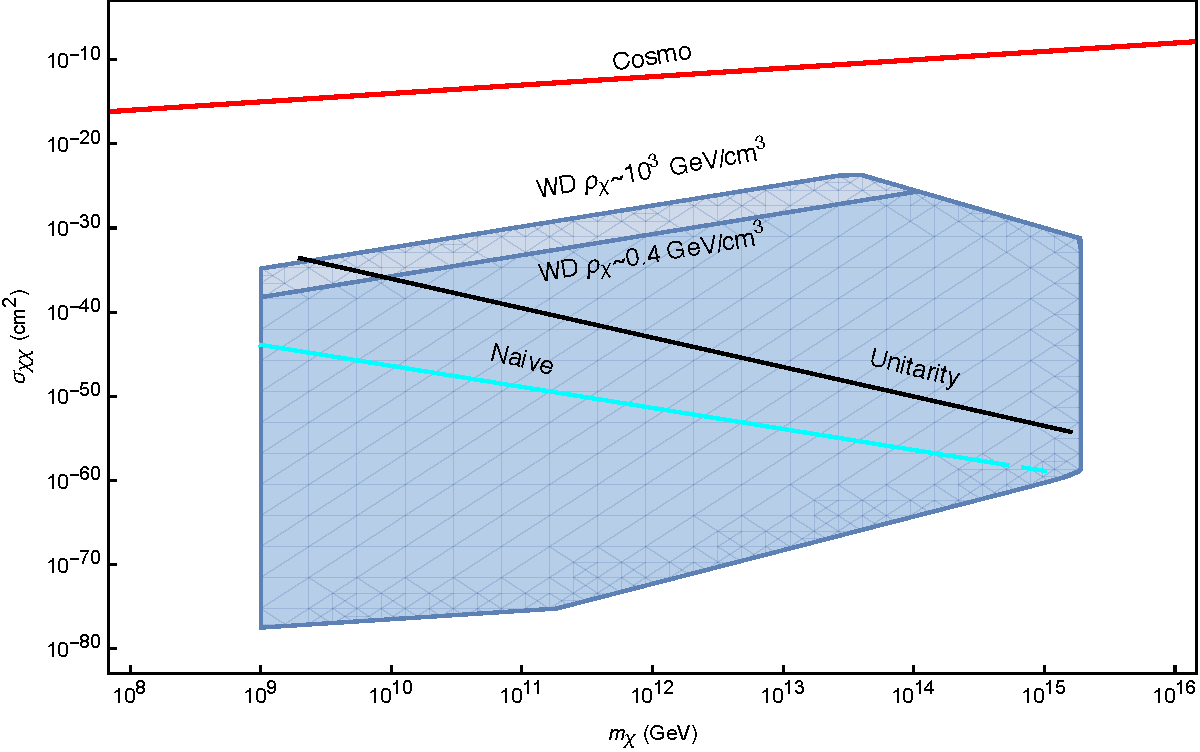
\includegraphics[scale=.35]{GZcapture.pdf}
\caption{Constraints on ``WIMPzilla" DM models which elastically scatter off nuclei through Z boson-exchange and annihilate to electroweak gauge bosons. Bounds come from observation of a single $1.25~M_{\astrosun}$ WD.
We assume the DM collapse is stabilized by formation of a BH. Also shown are the naive estimate (green) estimate and unitarity limit (blue) for this annihilation cross section.}
\label{fig:Gutzilla}
\end{figure}

\end{document}